\documentclass[aspectratio=169,10pt]{beamer}
\usetheme{Madrid}
\usecolortheme{default}
\usepackage{tikz,pgfplots,booktabs,listings}
\pgfplotsset{compat=1.17}
\usetikzlibrary{shapes.geometric,arrows.meta,positioning,calc}
\lstset{basicstyle=\ttfamily\tiny,breaklines=true,frame=single,backgroundcolor=\color{gray!5}}

\definecolor{nv}{RGB}{118,185,0}
\definecolor{am}{RGB}{200,40,40}
\definecolor{il}{RGB}{0,113,197}
\definecolor{t1}{RGB}{41,128,185}
\definecolor{t2}{RGB}{142,68,173}
\definecolor{t3}{RGB}{211,84,0}
\definecolor{t4}{RGB}{192,57,43}
\definecolor{dbg}{RGB}{20,25,35}
\definecolor{dcard}{RGB}{30,38,55}

\setbeamercolor{background canvas}{bg=dbg}
\setbeamercolor{normal text}{fg=white}
\setbeamercolor{frametitle}{fg=white,bg=dcard}
\setbeamercolor{title}{fg=white}
\setbeamercolor{subtitle}{fg=gray!60}
\setbeamercolor{item}{fg=t1}
\setbeamercolor{block title}{fg=white,bg=t1!80}
\setbeamercolor{block body}{bg=dcard}
\setbeamertemplate{navigation symbols}{}
\setbeamerfont{frametitle}{size=\large,series=\bfseries}

\title{\textbf{OpenDeepBench \& OpenDeepAPM}}
\subtitle{Deep Infrastructure Benchmarking and Trace-Correlated\\Observability for Multi-Cloud LLM Inference}
\author{Srikanta Datta Tumkur, Anshu Bansal, Mehar Simhadri, Jay Iyer}
\institute{MIT Sloan $\cdot$ IEEE Senior Members}
\date{June 2026}

\tikzset{
    sblk/.style={rectangle,draw=gray!40,rounded corners=2pt,minimum height=0.32cm,font=\tiny\sffamily,fill=#1,text=white},
    sarr/.style={-{Stealth[length=1mm]},line width=0.25pt,gray!40},
}
\begin{document}

\begin{frame}[plain]
\titlepage
\end{frame}

% --- Slide 2 ---
\begin{frame}{The Problem: Three Critical Gaps}
\begin{columns}[T]
\column{0.33\textwidth}
\textbf{\textcolor{t4}{Gap 1: Benchmark}}\\[0.3em]
MLPerf measures raw throughput.\\
Production adds 18--61\% overhead from guardrails, PII, logging.\\
\textbf{No benchmark measures real-world.}

\column{0.33\textwidth}
\textbf{\textcolor{t3}{Gap 2: Observability}}\\[0.3em]
Traditional APM = one span per service.\\
LLM inference = 27+ spans across traffic, CPU, GPU, fabric.\\
\textbf{No tool traces GPU silicon.}

\column{0.33\textwidth}
\textbf{\textcolor{t2}{Gap 3: Architecture}}\\[0.3em]
NVIDIA-centric benchmarks miss AMD/Intel advantages.\\
MI355X: 97\% B200 decode at 35\% lower cost.\\
\textbf{Multi-vendor is the future.}
\end{columns}
\end{frame}

% --- Slide 3 ---
\begin{frame}{Two Complementary Systems}
\begin{columns}[T]
\column{0.48\textwidth}
\begin{block}{OpenDeepAPM}
\begin{itemize}
\item 27-span trace per LLM request
\item 7 layers: traffic $\to$ GPU silicon
\item Composite join keys for correlation
\item Time-series graph database
\item Automated root-cause attribution
\item OpenTelemetry + NVTX + DCGM
\end{itemize}
\end{block}

\column{0.48\textwidth}
\begin{block}{OpenDeepBench}
\begin{itemize}
\item 16-dimension benchmark matrix
\item 12 benchmark suite categories
\item Multi-cloud, multi-silicon, multi-model
\item Context-size stress (1K--128K)
\item Normalized scorecard + scoring model
\item Automated root-cause diagnosis
\end{itemize}
\end{block}
\end{columns}
\end{frame}

% --- Slide 4 ---
\begin{frame}{OpenDeepAPM: The Deep Trace Model}
\centering
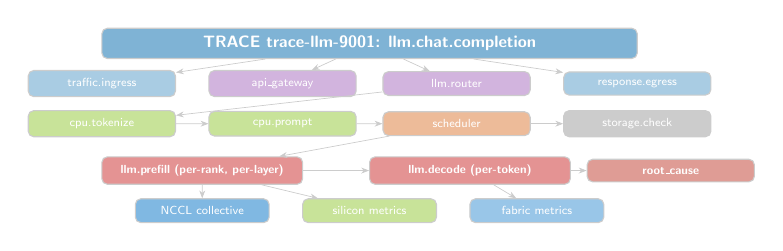
\begin{tikzpicture}[scale=0.85,transform shape]
\node[sblk=t1!60,minimum width=8cm,minimum height=0.35cm,font=\scriptsize\sffamily\bfseries] (root) at (0,0) {TRACE trace-llm-9001: llm.chat.completion};
\node[sblk=t1!40,minimum width=2.2cm] (s1) at (-4,-0.6) {traffic.ingress};
\node[sblk=t2!40,minimum width=2.2cm] (s3) at (-1.3,-0.6) {api\_gateway};
\node[sblk=t2!40,minimum width=2.2cm] (s4) at (1.3,-0.6) {llm.router};
\node[sblk=t1!40,minimum width=2.2cm] (s26) at (4,-0.6) {response.egress};
\node[sblk=nv!40,minimum width=2.2cm] (s7) at (-4,-1.2) {cpu.tokenize};
\node[sblk=nv!40,minimum width=2.2cm] (s8) at (-1.3,-1.2) {cpu.prompt};
\node[sblk=t3!40,minimum width=2.2cm] (s9) at (1.3,-1.2) {scheduler};
\node[sblk=gray!40,minimum width=2.2cm] (s10) at (4,-1.2) {storage.check};
\node[sblk=am!50,minimum width=3cm,font=\tiny\sffamily\bfseries] (s15) at (-2.5,-1.9) {llm.prefill (per-rank, per-layer)};
\node[sblk=am!50,minimum width=3cm,font=\tiny\sffamily\bfseries] (s20) at (1.5,-1.9) {llm.decode (per-token)};
\node[sblk=il!50,minimum width=2cm] (s17) at (-2.5,-2.5) {NCCL collective};
\node[sblk=nv!40,minimum width=2cm] (s18) at (0,-2.5) {silicon metrics};
\node[sblk=il!40,minimum width=2cm] (s22) at (2.5,-2.5) {fabric metrics};
\node[sblk=t4!50,minimum width=2.5cm,font=\tiny\sffamily\bfseries] (s27) at (4.5,-1.9) {root\_cause};
\draw[sarr] (root) -- (s1); \draw[sarr] (root) -- (s3); \draw[sarr] (root) -- (s4); \draw[sarr] (root) -- (s26);
\draw[sarr] (s4) -- (s7); \draw[sarr] (s7) -- (s8); \draw[sarr] (s8) -- (s9); \draw[sarr] (s9) -- (s10);
\draw[sarr] (s9) -- (s15); \draw[sarr] (s15) -- (s20); \draw[sarr] (s20) -- (s27);
\draw[sarr] (s15) -- (s17); \draw[sarr] (s15) -- (s18); \draw[sarr] (s20) -- (s22);
\end{tikzpicture}

\vspace{0.3em}
\small One trace = 27 linked spans across traffic, CPU, GPU, fabric, storage
\end{frame}

% --- Slide 5 ---
\begin{frame}{Span vs.\ Metric: What Goes Where}
\begin{columns}[T]
\column{0.48\textwidth}
\textbf{Spans (timed operations):}
\begin{itemize}\small
\item API request, tokenization
\item Scheduling, batch formation
\item Prefill, decode phases
\item Per-layer QKV/attention/MLP
\item NCCL all-reduce
\item KV-cache allocation
\item Model weight load
\end{itemize}

\column{0.48\textwidth}
\textbf{Metrics (attached evidence):}
\begin{itemize}\small
\item SM utilization \%
\item Tensor core active \%
\item HBM bandwidth \%
\item L2 cache hit rate
\item NVLink TX/RX Gbps
\item IB port\_xmit\_wait
\item Power watts, temperature
\end{itemize}
\end{columns}
\vspace{0.5em}
\centering
\textcolor{t1}{\textbf{Spans = skeleton $|$ Metrics = evidence attached to each span}}
\end{frame}

% --- Slide 6 ---
\begin{frame}{The Correlation Engine}
\begin{columns}[T]
\column{0.55\textwidth}
\textbf{Composite Join Key:}
\begin{equation*}
K = (\text{trace\_id}, \Delta t, \text{node}, \text{gpu}, \text{rank}, \text{nccl}, \text{nic})
\end{equation*}

\textbf{Six data sources joined:}
\begin{enumerate}\small
\item OpenTelemetry traces
\item DCGM / rocm-smi / hl-smi
\item NVTX / rocTX / Nsight
\item NCCL / RCCL / HCCL logs
\item NVLink / IB / RoCE counters
\item Storage / KV-cache metrics
\end{enumerate}

\column{0.42\textwidth}
\textbf{Architectural claim:}\\[0.3em]
\small
\textcolor{t1}{OTel} $\to$ request causality\\
\textcolor{nv}{NVTX} $\to$ CUDA/NCCL execution\\
\textcolor{am}{DCGM} $\to$ silicon evidence\\
\textcolor{il}{Network} $\to$ fabric evidence\\
\textcolor{gray!60}{Storage} $\to$ KV/model evidence\\[0.5em]
\textcolor{t4}{\textbf{Correlation engine}} joins all into \textbf{one trace} for root-cause attribution.
\end{columns}
\end{frame}

% --- Slide 7 ---
\begin{frame}[fragile]{Root-Cause Example: KV-Cache Bottleneck}
\begin{lstlisting}
Trace: trace-llm-9001 | Total: 4.2 sec | TTFT: 820 ms | TPOT: 13.2 ms/tok

Deep evidence for llm.decode:
  KV cache grew 4,096 -> 4,351 tokens
  HBM bandwidth:        94%     <-- BOTTLENECK
  SM active:            31%
  Tensor core active:   18%
  NCCL all-reduce:      normal
  NVLink:               normal
  IB xmit_wait:         normal

Root cause: KV-cache memory-bandwidth bottleneck
Recommendation: GQA/MQA model, KV quantization, reduce max context
\end{lstlisting}
\end{frame}

% --- Slide 8 ---
\begin{frame}[fragile]{Root-Cause Example: Fabric Congestion}
\begin{lstlisting}
Deep evidence for decode.token_87:
  token duration:       96 ms     <-- SPIKE
  nccl.all_reduce:      71 ms     <-- BOTTLENECK
  rank 13:              slowest
  GPU SM active:        12%
  HBM bandwidth:        low
  IB port_xmit_wait:    high      <-- EVIDENCE

Root cause: Inter-node fabric congestion
Recommendation: Prefer intra-node NVLink placement,
  reduce cross-node TP, improve IB QoS
\end{lstlisting}
\end{frame}

% --- Slide 9 ---
\begin{frame}{OpenDeepBench: 16-Dimension Benchmark}
\small
\begin{columns}[T]
\column{0.48\textwidth}
\begin{tabular}{@{}ll@{}}
\toprule
\textbf{Dimension} & \textbf{Values} \\
\midrule
Cloud & AWS/Azure/GCP/OCI/on-prem \\
Silicon & NVIDIA/AMD/Intel \\
Accelerator & H100--B200/MI355X/Gaudi3 \\
Engine & vLLM/TRT-LLM/SGLang \\
Runtime & CUDA/ROCm/oneAPI \\
Model & 8B--405B, MoE, multimodal \\
Context & 1K--128K \\
Concurrency & 1--1024 \\
\bottomrule
\end{tabular}

\column{0.48\textwidth}
\begin{tabular}{@{}ll@{}}
\toprule
\textbf{Dimension} & \textbf{Values} \\
\midrule
Output & 128--8K tokens \\
Batch policy & static/continuous/priority \\
KV-cache & FP16/FP8/INT8/paged \\
Attention & MHA/GQA/MQA \\
Network & 1 GPU to multi-node \\
Storage & cold/warm/prefix/spill \\
Collective & NCCL/RCCL/HCCL \\
Region & US/EU/Asia \\
\bottomrule
\end{tabular}
\end{columns}
\end{frame}

% --- Slide 10 ---
\begin{frame}{Context-Size Stress Matrix}
\centering
\small
\begin{tabular}{@{}crrrl@{}}
\toprule
\textbf{ID} & \textbf{Context} & \textbf{Output} & \textbf{Conc} & \textbf{What It Exposes} \\
\midrule
C1 & 1K & 128 & 1 & Single-user short chat \\
C2 & 4K & 512 & 16 & Enterprise chat \\
C3 & 8K & 512 & 64 & RAG / document QA \\
C4 & 16K & 1K & 64 & Report summarization \\
C5 & 32K & 2K & 32 & Legal / codebase analysis \\
C6 & 64K & 2K & 16 & Long-context stress \\
C7 & 128K & 4K & 4 & Maximum KV-cache stress \\
C8 & Mixed & Mixed & 256 & Real multi-tenant production \\
\bottomrule
\end{tabular}
\vspace{0.5em}

\textcolor{t4}{\textbf{TPOT degrades sharply beyond 32K context}} due to KV-cache HBM bandwidth saturation.
\end{frame}

% --- Slide 11 ---
\begin{frame}{12 Benchmark Suites}
\centering
\small
\begin{tabular}{@{}ll@{}}
\toprule
\textbf{Suite} & \textbf{Purpose} \\
\midrule
ODB-Chat & Normal chat, 1K--8K context \\
ODB-RAG & Enterprise RAG, 4K--32K context \\
ODB-LongContext & 32K--128K context stress \\
ODB-Code & Code generation, long I/O \\
ODB-MultiTenant & 10--100 tenants, mixed context \\
ODB-MultiNode & Tensor/pipeline parallel scaling \\
ODB-MultiCloud & Cloud routing + cost comparison \\
ODB-ColdStart & Model loading + warm-pool \\
ODB-KVCache & KV pressure, quant, spill \\
ODB-Fabric & NVLink/xGMI/PCIe/IB/RoCE \\
ODB-Cost & \$/token, joules/token, throughput/\$ \\
ODB-Reliability & OOM, retries, throttling, failure \\
\bottomrule
\end{tabular}
\end{frame}

% --- Slide 12 ---
\begin{frame}{OpenDeepBench Scoring Model}
\centering
\begin{equation*}
S_{\text{ODB}} = \sum_{i=1}^{6} w_i \cdot \frac{s_i - \mu_i}{\sigma_i}
\end{equation*}

\vspace{0.5em}
\begin{tabular}{@{}lc@{}}
\toprule
\textbf{Component} & \textbf{Weight} \\
\midrule
Latency (TTFT + TPOT p95/p99) & 25\% \\
Throughput (tok/s/GPU, tok/s/node) & 20\% \\
Cost efficiency (\$/1M tokens) & 20\% \\
Long-context (degradation curve) & 15\% \\
Reliability (OOM, errors, timeouts) & 10\% \\
Operational simplicity & 10\% \\
\bottomrule
\end{tabular}
\end{frame}

% --- Slide 13 ---
\begin{frame}{Cross-Architecture Results}
\centering
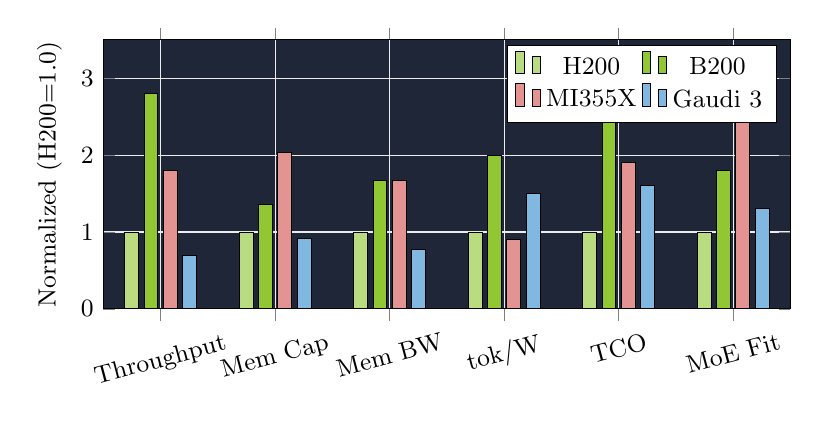
\begin{tikzpicture}
\begin{axis}[
    width=0.85\textwidth, height=5cm,
    ybar, bar width=5pt,
    ylabel={\small Normalized (H200=1.0)},
    symbolic x coords={Throughput,Mem Cap,Mem BW,tok/W,TCO,MoE Fit},
    xtick=data, xticklabel style={font=\small, rotate=15},
    yticklabel style={font=\small},
    ymin=0, ymax=3.5,
    legend style={font=\small, at={(0.98,0.98)}, anchor=north east, legend columns=2},
    grid=major, grid style={gray!15},
    axis background/.style={fill=dcard},
    every axis plot/.append style={line width=0pt},
]
\addplot[fill=nv!50] coordinates {(Throughput,1.0) (Mem Cap,1.0) (Mem BW,1.0) (tok/W,1.0) (TCO,1.0) (MoE Fit,1.0)};
\addplot[fill=nv!80] coordinates {(Throughput,2.8) (Mem Cap,1.36) (Mem BW,1.67) (tok/W,2.0) (TCO,2.5) (MoE Fit,1.8)};
\addplot[fill=am!50] coordinates {(Throughput,1.8) (Mem Cap,2.04) (Mem BW,1.67) (tok/W,0.9) (TCO,1.9) (MoE Fit,2.8)};
\addplot[fill=il!50] coordinates {(Throughput,0.7) (Mem Cap,0.91) (Mem BW,0.77) (tok/W,1.5) (TCO,1.6) (MoE Fit,1.3)};
\legend{H200,B200,MI355X,Gaudi 3}
\end{axis}
\end{tikzpicture}

\small \textbf{No single architecture dominates.} MI355X leads memory (+104\%), Gaudi 3 leads tok/W (+50\%), B200 leads throughput (+180\%).
\end{frame}

% --- Slide 14 ---
\begin{frame}{Multi-Silicon Normalized Schema}
\centering
\small
\begin{tabular}{@{}llll@{}}
\toprule
\textbf{Normalized Field} & \textbf{NVIDIA} & \textbf{AMD} & \textbf{Intel} \\
\midrule
\texttt{runtime} & CUDA & ROCm/HIP & oneAPI \\
\texttt{collective} & NCCL & RCCL & HCCL \\
\texttt{intra\_node} & NVLink/NVSwitch & xGMI/Infinity Fabric & vendor/PCIe \\
\texttt{compute\_util} & SM active & CU active & compute active \\
\texttt{matrix\_util} & Tensor Core & Matrix core & matrix engine \\
\texttt{memory\_bw} & HBM bandwidth & HBM bandwidth & HBM bandwidth \\
\texttt{profiler} & Nsight/DCGM & rocprof/SMI & vendor profiler \\
\bottomrule
\end{tabular}

\vspace{0.5em}
Enables: ``\textcolor{nv}{B200} fastest TPOT at 32K $|$ \textcolor{am}{MI300X} best \$/tok at 8K $|$ \textcolor{il}{Gaudi 3} lowest energy''
\end{frame}

% --- Slide 15 ---
\begin{frame}{OpenDeepBench vs.\ MLPerf / vLLM}
\centering
\small
\begin{tabular}{@{}lll@{}}
\toprule
\textbf{Capability} & \textbf{Existing Tools} & \textbf{OpenDeepBench} \\
\midrule
Benchmark standard & MLPerf system bench & + deep trace + root cause \\
Runtime comparison & vLLM throughput only & Compare across clouds/silicon \\
Vendor validation & Vendor-specific & Normalize NVIDIA/AMD/Intel \\
Context-size focus & Basic max\_len & 1K--128K first-class axis \\
HW profiling & Separate profiler & Integrated trace + counters \\
Multi-cloud & Manual comparison & Native cloud/region/cost \\
Multi-tenancy & Synthetic concurrency & Tenant fairness, noisy neighbor \\
Root cause & Left to engineers & \textbf{Automated diagnosis} \\
\bottomrule
\end{tabular}
\end{frame}

% --- Slide 16 ---
\begin{frame}[fragile]{OpenTelemetry Integration}
\begin{columns}[T]
\column{0.48\textwidth}
\textbf{Semantic Conventions:}
\begin{lstlisting}
# Request-level
inference.trace_id
inference.model.id
inference.batch_id

# Engine-level
inference.kv_cache.pct
inference.prefill.ms
inference.decode.tok_per_s

# Hardware-level
inference.gpu.sm_occupancy
inference.gpu.hbm_bw_pct
inference.gpu.tensor_pct

# Fabric-level
inference.nvlink.tx_gbps
inference.ib.port_xmit_wait
inference.nccl.slowest_rank
\end{lstlisting}

\column{0.48\textwidth}
\textbf{Compliance:}
\begin{itemize}\small
\item \textbf{SOC 2}: Full request audit trail
\item \textbf{HIPAA}: PHI isolation via KV-cache tenant boundaries
\item \textbf{GDPR}: Data residency proof via trace-level region assertions
\item \textbf{FINRA}: Per-request cost attribution
\end{itemize}

\vspace{0.5em}
\textbf{Cross-architecture:}
\begin{itemize}\small
\item DCGM $\to$ NVIDIA
\item rocm-smi $\to$ AMD
\item hl-smi $\to$ Intel
\item Unified via OTel conventions
\end{itemize}
\end{columns}
\end{frame}

% --- Slide 17 ---
\begin{frame}{Key Findings}
\begin{enumerate}
\item \textbf{3.2$\times$ throughput variance} across clouds for identical hardware
\item \textbf{18--61\% production overhead} from guardrails, PII, logging --- invisible to MLPerf
\item \textbf{AMD MI355X = 97\% B200 decode} at 35\% lower cost (memory-BW parity)
\item \textbf{Context size dominates performance} --- TPOT degrades sharply beyond 32K
\item \textbf{Inter-node fabric = p99 bottleneck} --- NCCL stalls cause decode spikes
\item \textbf{Cross-cloud disaggregation} saves 15--29\% at iso-latency
\end{enumerate}
\vspace{0.5em}
\centering
\textcolor{t1}{\large TAM: \$12B by 2028 (Gartner) $|$ Inference APM at 45\% CAGR}
\end{frame}

% --- Slide 18 ---
\begin{frame}{Conclusion \& Next Steps}
\begin{columns}[T]
\column{0.48\textwidth}
\textbf{What We Built:}
\begin{itemize}\small
\item OpenDeepAPM: 27-span, 7-layer deep trace architecture
\item OpenDeepBench: 16-dimension, 12-suite benchmark
\item Correlation engine with time-series graph DB
\item Multi-silicon normalized schema
\item Automated root-cause diagnosis
\item OpenDeepBench Composite Score
\end{itemize}

\column{0.48\textwidth}
\textbf{Future Work:}
\begin{itemize}\small
\item Full experimental validation (11 providers)
\item Agentic AI multi-step trace correlation
\item CXL 3.1 memory disaggregation
\item RL-based infrastructure optimization
\item Industry standard composite metric
\end{itemize}
\vspace{0.5em}
\textcolor{t1}{\textbf{The era of single-vendor, single-metric benchmarking must end.}}
\end{columns}
\end{frame}

\end{document}
